\setcounter{chapter}{5}
\chapter{\acs{fastPLI}}
\label{chap:Software}
% 
% \cleanchapterquote{There are only two kinds of languages: the ones people complain about and the ones nobody uses.}{Bjarne Stroustrup}{The \cpp{} Programming Language}
% 
% 
\includegraphics[width=.075\textwidth]{gfx/Scihub_raven.png}
% \cleanchapterquote{Journal paywalls are an example of something that works in the reverse direction, making communication less open and efficient.}{Alexandra Elbakyan}{}
% % 
% % \tikz[remember picture,overlay] \node[inner sep=0pt] at (0,0){
\includegraphics[height=7em]{gfx/Scihub_raven.png}};
% % \hspace{-10em}
% % \clearpage opacity=0.3,
% 
% 
%  
\section{Introduction}\label{sec:fastpliIntro}
% 
In the previous chapters, the algorithms for creating dense \ac{WM} fiber models (see \cref{chap:sof:modelling}) and simulating \ac{3D-PLI} (see \cref{cha:sof:simulation}) are described.
Both algorithms are designed to work without knowledge of the other.
This allows \eg{} to be useful for models in other domains, such as \ac{dMRI} (\cite{Ginsburger2019,ginsburgerDis2019}).
However, in addition to providing algorithms that are intended to be very fast and thus as in this case at a very low level, it is also necessary to provide an \ac{API} that provides an interface to the user.
This interface must be designed in such a way that the user has a good experience when working with the algorithms.
Among other things, this means a high level of abstraction with logical and easy-to-use naming systems.
A high level of abstraction in software design means that unnecessary systems and generalizations of functionalities are hidden.
% 
\par
% 
In addition, the algorithms should be accessible to a wide audience.
Among other things, this means that the program must be installable and easy to understand, even if no programming knowledge is available.
The latter is of course a problem, however, in the last decades more and more higher programming languages have been designed to be easily understandable.
% 
\par
% 
For the above reasons, the \python{} programming language was chosen.
It has become increasingly popular in the last decade, especially in data science.
The core algorithms remain in \cpp{} as described in their chapters to ensure efficiency, speed and parallelization.
%
\section{Toolbox}
% 
\begin{figure}[!ht]
\centering
% \resizebox{0.95\textwidth}{!}{
% \setlength{\tikzwidth}{0.75\textwidth}
\inputtikz{gfx/fastpli/fastpli_pipeline}
% }
\caption[\acs{fastPLI}]{\ac{fastPLI} package structure}
\label{fig:fastpli}
\end{figure}
% 
The \python{} package is called \ac{fastPLI}.
Its source code is publicly available and \cite{fastpli,Matuschke2021} published.
The software package includes functionalities for the analysis and visualization of the nerve fiber models as well as for the analysis of the simulation analogous to the current routine experimental measurements, \eg{} tilting analysis.
% 
% 
% 
\subsection{Documentation}
% 
\begin{figure}[!t]
    \centering
    \resizebox{\textwidth}{!}{\fbox{
    \begin{tabular}{c|c}
    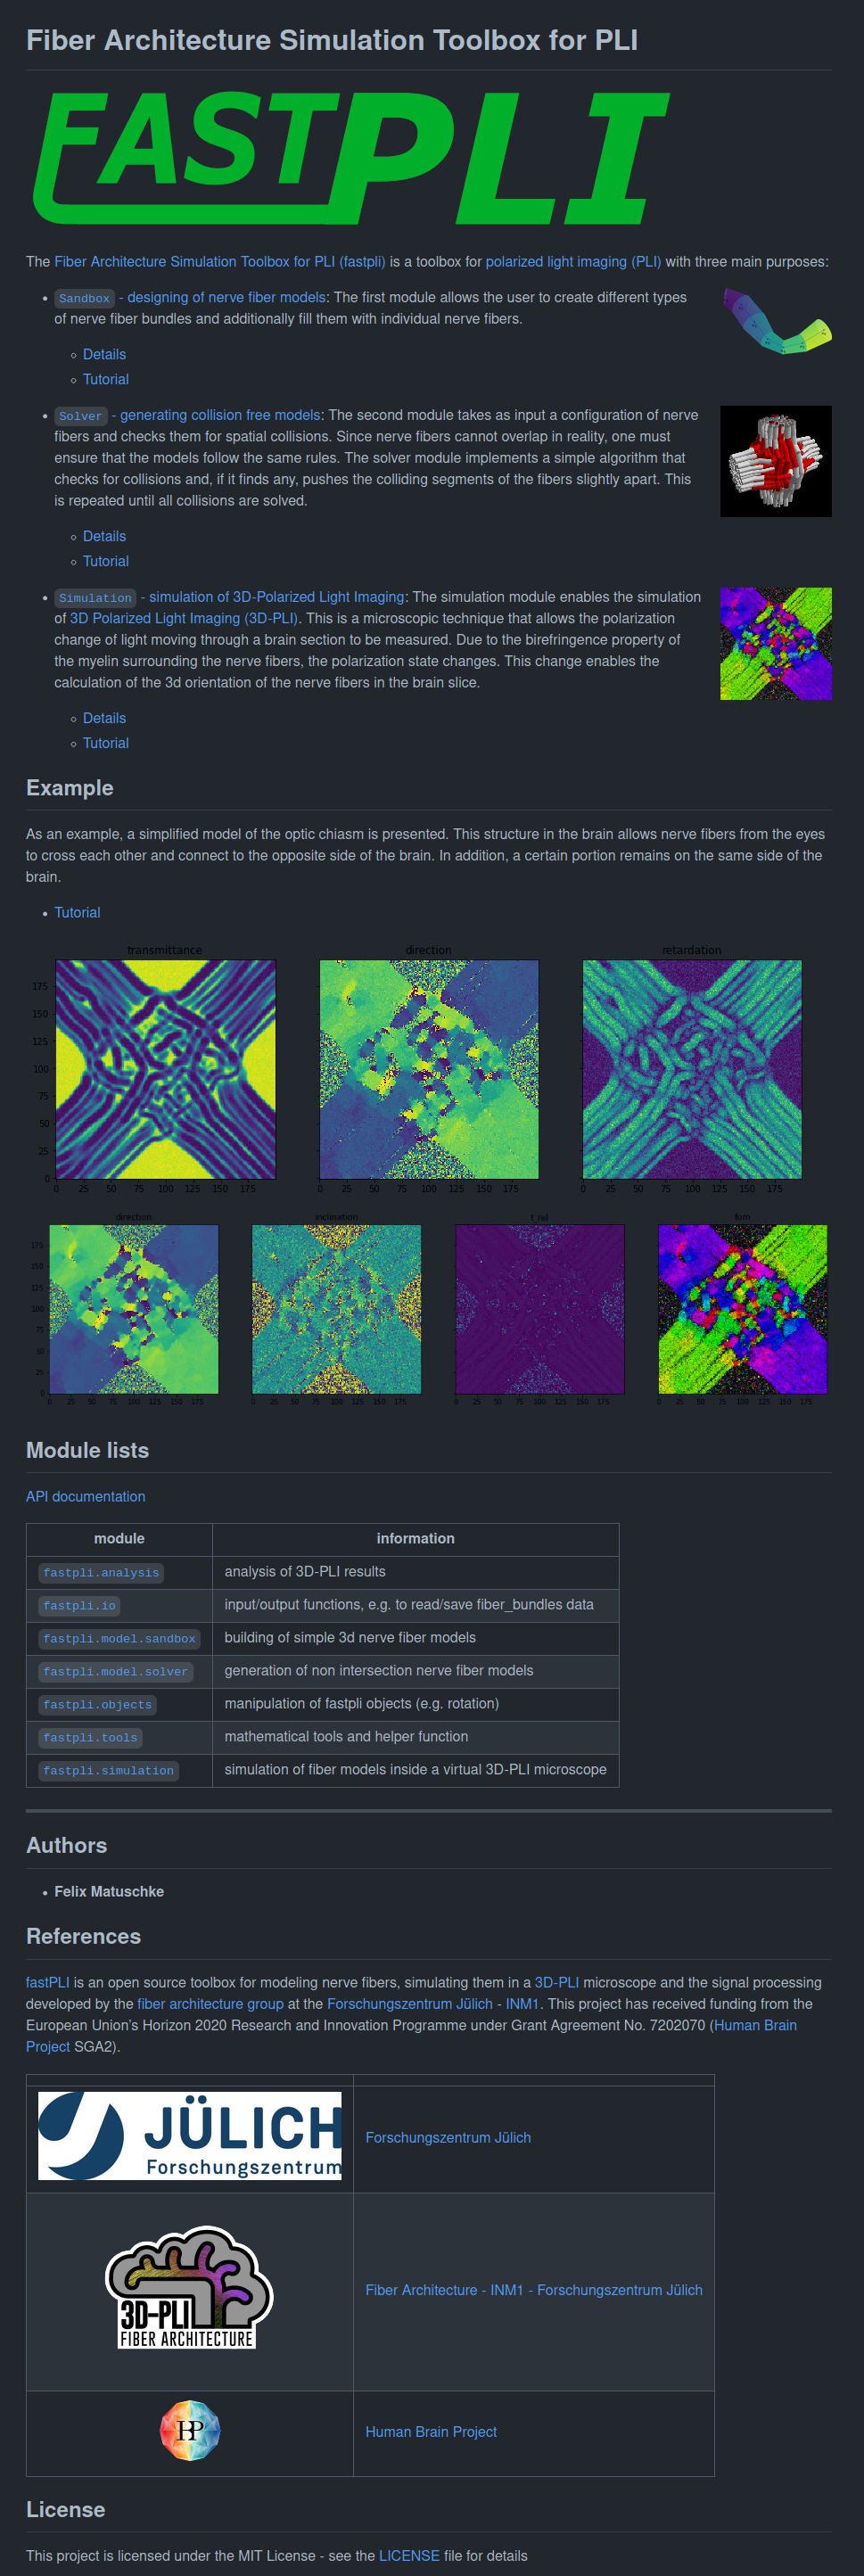
\includegraphics[valign=T,trim=0 1300 0 0, clip]{gfx/fastpli/fastpli_wiki.png} &
 	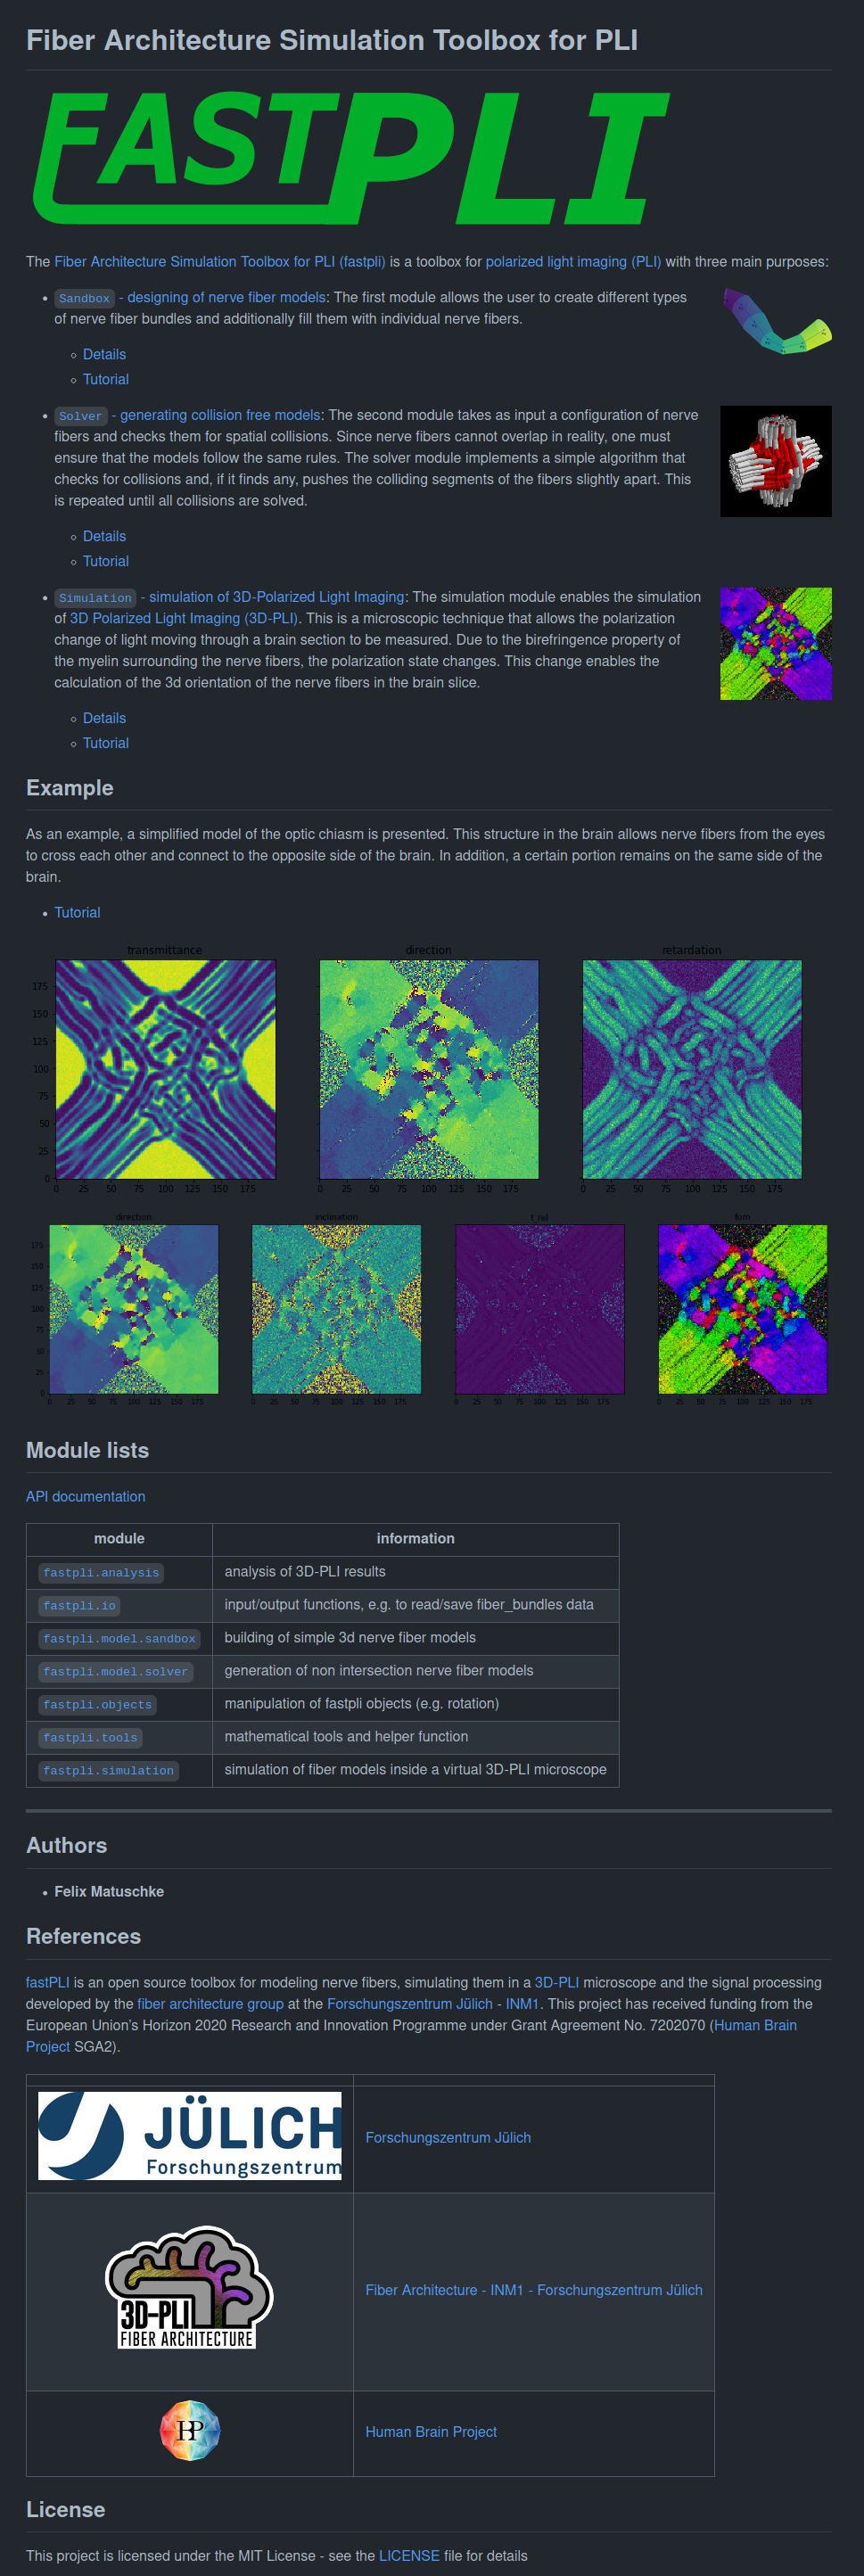
\includegraphics[valign=T,trim=0 0 0 1580, clip]{gfx/fastpli/fastpli_wiki.png} \\
    \end{tabular}
    }}
	\caption[Documentation]{Documentation Wiki Page of the Github repository \url{https://github.com/3d-pli/fastpli/wiki}.}
	\label{fig:fastpli_wiki}
\end{figure}
% 
As is common in software development, all methods are provided with docstrings (documentation string) to help the user understand how they work.
These are displayed e.g. by modern editors automatically wäres during programming, in order to give assistance.
These docstrings are also used for an automatic release of a \ac{API} documentation.\footnote{\url{https://3d-pli.github.io/fastpli/}}
In addition, a wiki page (see \cref{fig:fastpli_wiki}) describing the main features is available, which is an essential part of the review process for publication in \textit{the Journal of Open Source Software (JOSS)} \cite{Matuschke2021}. \footnote{review openly accessible at \url{https://github.com/openjournals/joss-reviews/issues/3042}}
The wiki page is structured as a guide leading through the aspect of designing nerve fiber models, applying the collision solving algorithm, the visualization of nerve fibers, a simple guide to \ac{3D-PLI} and finally the application of the models in the simulation.
To help users get started quickly, both executable \python{} scripts and Jupyter notebooks are available as tutorials.
A combined example for the whole package based on the optical chiasm, the nerve fiber crossing of the optical path from eyes to occipital lobe, is accessible as the last part.
% 
% 
% 
\subsection{Dependencies}
% 
\paragraph{Python:}
\begin{description}
\item[numpy:] Base N-dimensional array package \cite{2019arXiv190710121V}\\
\url{https://numpy.org/}
\item[scipy:] Fundamental library for scientific computing \cite{2019arXiv190710121V}\\
\url{https://www.scipy.org/} 
\item[numba:] Acceleration of Python Functions \cite{Lam2015}\\
\url{https://numba.pydata.org/}
\item[mpi4py:] MPI for Python \cite{Dalcn2005, Dalcn2008, Dalcin2011}\\
\url{https://bitbucket.org/mpi4py/mpi4py/src/master/}
\item[h5py:] HDF5 for Python \cite{collette_python_hdf5_2014, hdf5}\\
\url{https://www.h5py.org/}
\end{description}
% 
\paragraph{C++:}
\begin{description}
\item[MPI:] Message Passing Interface \cite{message2015mpi}\\
\url{https://www.mpi-forum.org/}
\item[OpenMP:] Open Multi-Processing, API for multi-platform shared memory multiprocessing programming \cite{dagum1998openmp}\\
\url{https://www.openmp.org/}
\item[OpenGL:] Open Graphics Library \cite{khronos}\\
\url{www.opengl.org}
\item[Pybind11:] Seamless operability between C++11 and Python \cite{pybind11}\\ \url{https://github.com/pybind/pybind11} 
\end{description}
%
% 
At this point, only Linux builds are supported.
However, for current Windows versions, the \ac{WSL} provides a fully functional Linux kernel inside Windows.
This makes it possible to run the same software as under native linux distributions.
Current macOS versions are not supported, but due to the minimalistic style of the \ac{fastPLI} package, the required changes should be feasible with minimal modifications.
% 
% 
% 
\subsection{Installation}
% 
The installation is handled by a \name{Makefile}.
It first starts a \name{CMake} routine, which searches for all necessary libraries and programms.
Then the \cpp{} code will be compiled and the resulting \name{shared object libraries} will stored inside the \python{} routines.
This allows \python{} to install the package into the users environment.
% 
\begin{lstfloat}[!ht]
\lstset{style=common}
\begin{lstlisting}
make fastpli
pip3 install .
\end{lstlisting}
\end{lstfloat}
% 
% 
% 
\subsection{Tests/Verification/Issues}
% 
To provide fully tested software, each module with its main methods is automatically tested after each push\footnote{uploud of an \textit{git} commit} with a Github actiontested. \footnote{Github actions are commenly used for automatic build, test and deployment of the software and documentation} 
This action runs the two latest Ubuntu Long Term Support versions (18.04 LTS and 20.04 LTS) and the most commonly used Python3 versions (3.6 and 3.8) to provide a wide range of supported common versions.
In addition, the \textit{Github actions} run all test scripts, check tutorial files, check code format and linting for consistency, and publish the latest documentation.
% 
\par
% 
Github allows to track \name{Issues}.
This feature originally is used to document software bugs.
However it is also used to discuss ideas, new features and so on.
In context of the open source publication, it was also used to discuss the review.
This allows to always additionally with the git \name{commits} to trace back the development process and code changes.
%
%  
% 
%  
\section{modules}
% 
A \python{} package consist out of modules, which contain the definitions of functions, classes and so on.
In the following the different modules will be listed alphabetically.
% 
% 
% 
\subsection{\Code{fastpli.analysis}}
% 
This module contains all functionalities to analyse the \ac{3D-PLI} simulations analog to the routine measurements.
This includes the analysis of the signal to the three image modalities transmittance, direcion and retardadation.
Further it provides the tilting analysis known as \ac{ROFL} \cite{Schmitz2018}.
The final helper functions provides methods to convert the direction and inclination results into a \ac{FOM}.
\\
For the analysis of fiber models, the module providing a few simple helper functions.
This for example allow the user to generate a histogramm of the orientations of the fiber segments like the ones shown in this thesis.
% 
\subsection{\Code{fastpli.io}}
% 
This methods provides the reading and writing routines to allow the user to read and save fiber models (\ie{} \code{fiber\_bundles}) to or from the disk.
There are two formats available.
The first one is a simple text file with the extension \code{.dat} (see \cref{alg:dat-file}).
Here each $(x,y,z,r)$ tuple of a fiber point is stored as a single line in the file.
Two fibers are seperated via an empty line while two fiber bundles are seperated via two empty lines.
This dataformat is provided to allow a very easy format to manipulate, exchange and read the files \eg{} into other programms.
% 
\begin{lstfloat}[!ht]
\lstset{style=common,morecomment=[l][\color{syntax_green}]{##},}
\begin{lstlisting}
-6.55 -18.93 -64.98 3.75 # x y z r
-5.73 -14.89 -63.37 3.4
-4.42 -13.66 -58.95 3.05
    # empty line indicates new fiber
-1.96 -10.07 -52.5 2.92
-1.03 -9.4 -48.62 2.93

    # two empty lines indicates new fiber bundle
3.4 -4.02 -44.76 3.11
6.22 -1.04 -42.45 3.26
\end{lstlisting}
\caption{exemplary dat-file format. Commets are currently not allowed and are only for the readers eyes.}\label{alg:dat-file}
\end{lstfloat}
% 
% 
\par
The second format uses \hdf{} \cite{hdf5}, which uses a binary dataformat.
\hdf{} allows to store the data as \code{datasets} into \code{groups}.
This is analog to a file in a operating systems, which is stored into folders.
The \hdf{} groups are used to store the \code{fiber} into \code{fiber\_bundle} and \code{fiber\_bundles}.
The $(x,y,z,r)$ informations of each fiber is then stored as 2d array (see \cref{alg:hdf5}). 
% 
\begin{lstfloat}[!ht]
\lstset{style=common,morecomment=[l][\color{syntax_green}]{##},}
\begin{lstlisting}
GROUP "/" { # fiber_bundles path
  GROUP "0" { # id of fiber_bundle
      DATASET "0" { # id of fiber
         DATATYPE  H5T_IEEE_F64LE
         DATASPACE  SIMPLE { ( 3, 4 ) / ( 3, 4 ) }
         DATA {
         (0,0): -6.55, -18.93, -64.98, 3.75,
         (1,0): -5.73, -14.89, -63.37, 3.4,
         (2,0): -4.42, -13.66, -58.95, 3.05,
         }
      }
      DATASET "1" { # id of fiber
         DATATYPE  H5T_IEEE_F64LE
         DATASPACE  SIMPLE { ( 2, 4 ) / ( 2, 4 ) }
         DATA {
         (0,0): -1.96, -10.07, -52.5, 2.92,
         (1,0): -1.03, -9.4, -48.62, 2.93,
         }
      }
  }
  GROUP "1" { # id of fiber_bundle
      DATASET "0" { # id of fiber
         DATATYPE  H5T_IEEE_F64LE
         DATASPACE  SIMPLE { ( 2, 4 ) / ( 2, 4 ) }
         DATA {
         (0,0): 3.4, -4.02, -44.76, 3.11,
         (1,0): 6.22, -1.04, -42.45, 3.26,
         }
      }
  }
}
\end{lstlisting}
\caption{exemplary fiber format in \hdf{}.} \label{alg:hdf5}
\end{lstfloat}
% 
% 
% 
\subsection{\Code{fastpli.model.sandbox}}
% 
This module provides all the functionalities described in \cref{sec:sandbox}.
The module is split in two submodules: \code{fastpli.sandbox.build} and \code{fastpli.sandbox.seeds}.
The \code{fastpli.sandbox.seeds} includes all methods to populate a 2d-plane as described in \cref{sec:seeds}.
To populate the fiber from the seeds, the module \code{sandbox.build} provides the methods.
This include all described functions from \cref{sec:fillBundle}.
% 
% 
% 
\subsection{\Code{fastpli.model.solver}}
% 
The \code{fastpli.model.solver} module contains the compiled solving algorithm explained in detail in \crefrange{sec:Solver}{sec:modelOpt}.
Additionally the solver algorithm is wrapped inside the class \code{fastpli.model.solver.Solver}.
This wrapper class provides a higher level of abstraction (see \cref{sec:fastpliIntro}).
It contains all necessary variables as attributes and provides therefore an read/write access via class properties, \eg{} \code{Solver.obj\_mean\_length = } \dummy{}.
Every write method checks the input for user errors and provides a error message.
This class also contains a \code{Solver.get\_dict()} method, which returns a \python{} dictionary containing all variables and there values for reproducability.
It is also possible to save the class state, with the current state of the \code{fiber\_bundles}, as a \hdf{} object.
Finally this class also provides an easy use of a simple visualization (see \cref{sec:visualization}) of the solving process.
% 
% 
% 
\subsection{\Code{fastpli.objects}}
%
This modules provides wrapper class for \code{fastpli.objects.fibers} and \code{fastpli.objects.layers}.
Essentially \code{layers} are a \code{list} of \code{layer}, which themself are a \code{tuple} of the 4 attributes \code{absorption}, \code{birefringence}, \code{model} and \code{scale} (see \cref{sec:dv_generator}).
This wrapper class contains attributes which allows the user to acces this values by there name, instead of the \code{tuple} index \code{[i]}.
This is helpful to reduce user errors.
\\
The same is acomblished for \code{fastpli.objects.fibers}, which contain \code{fastpli.objects.FiberBundles}, \code{fastpli.objects.FiberBundle} and \code{fastpli.objects.Fiber} classes with the same purpase.
\code{FiberBundles} are a \code{list} of \code{FiberBundle}, which are a list of \code{Fiber}.
The data of a fiber is stored in a \code{numpy.ndarray}, which stores the values contiguous in memory.
Manipulation methods are provided for each class to allow the user to \code{translate}, \code{rotate}, \code{scale} and \code{cut} the model.
The letter helps especially in the solving process to reduce the number of objects, if only a certain volume shell be generated (since the solving process pushes the fiber objects apart and therefore increasing the volume).
% 
% 
% 
\subsection{\Code{fastpli.simulation}}
Like the \code{fastpli.model.solver.Solver} class this method provides a wrapper for the simulation called \code{fastpli.simulation.Simpli} based on the original algorithm \cite{Dohmen2015,Lucksch2016}.
It contains both algorithms \code{Generator} and \code{Simulation} described in \cref{sec:dv_generator,sec:simulation}.
These two algorithms work seperatly, however since they share quite a few parameters, they coexists inside the class.
As in the \code{fastpli.model.solver.Solver} class, all necessary attributes are available and are checked for input errors.
Since the analysis is usually always performed on the resulting simulations, they are also available in this class and performed with the same defined parameters as in the simulation.
Methods to save the variables as \code{dict} or \hdf{} files are available as well.
\\
As in the experiment, the simulations can run the same routine.
This means, that many parameters and the simulation pipeline usually does not change.
For this purpose \code{pipeline} methods exists (see \cref{alg:Pipeline}), to provide a high level abstraction.
Here all data is automatically analysed and saved and only the parameters have to be specified.
% 
\begin{lstfloat}[!tb]
\centering
\scalebox{0.75}{
\begin{minipage}{\the\textwidth}
\lstinputlisting[style=python]{code/pipeline.py.tex}
\end{minipage}}
\caption{Simulation pipeline}
\label{alg:Pipeline}
\end{lstfloat}
% 
% 
\subsection{\Code{fastpli.tools}}
The last module contains a variety of helper functions.
They provide access to the current version as well as to the git hash, so that any calculations can be reproduced.
For the fiber modelling rotation matrices are provided, to allow the usage of linear algebra.
% 
% 
% 
% \par
% \noindent\rule{\textwidth}{2pt}
% \newpage
